\documentclass[letterpaper,11pt]{article}
\oddsidemargin -1.0cm \textwidth 17.5cm

\usepackage[utf8]{inputenc}
\usepackage[activeacute,spanish, es-lcroman]{babel}
\decimalpoint
\usepackage{amsfonts,setspace}
\usepackage{amsmath}
\usepackage{amssymb, amsmath, amsthm}
\usepackage{comment}
\usepackage{float}
\usepackage{amssymb}
\usepackage{dsfont}
\usepackage{anysize}
\usepackage{multicol}
\usepackage{enumerate}
\usepackage{graphicx}
\usepackage[left=1.5cm,top=2cm,right=1.5cm, bottom=1.7cm]{geometry}
\setlength\headheight{1.5em} 
\usepackage{fancyhdr}
\usepackage{multicol}
\usepackage{hyperref}
\usepackage{wrapfig}
\usepackage{subcaption}
\usepackage{siunitx}
\usepackage{cancel}
\usepackage{mdwlist}
\usepackage{svg}
\pagestyle{fancy}
\fancyhf{}
\renewcommand{\labelenumi}{\normalsize\bfseries P\arabic{enumi}.}
\renewcommand{\labelenumii}{\normalsize\bfseries (\alph{enumii})}
\renewcommand{\labelenumiii}{\normalsize\bfseries \roman{enumiii})}


\begin{document}

\fancyhead[L]{\itshape{Facultad de Ciencias F\'isicas y Matem\'aticas}}
\fancyhead[R]{\itshape{Universidad de Chile}}

\begin{minipage}{11.5cm}
    \begin{flushleft}
        \hspace*{-0.6cm}\textbf{FI1000-6 Introducción a la Física Clásica}\\
        \hspace*{-0.6cm}\textbf{Profesora:} Paulina Lira\\
        \hspace*{-0.6cm}\textbf{Auxiliares:} Juan Cristóbal Castro \& Alejandro Silva\\
        \hspace*{-0.6cm}\textbf{Ayudantes:} Francisca Bórquez, Catalina Molina \& Erick Pérez\\
        
    \end{flushleft}
\end{minipage}

\begin{picture}(2,3)
    \put(366, 10){
\includegraphics[scale=0.9]{2020-1/Imágenes/logo/dfi-fcfm.pdf}}
\end{picture}

\begin{center}
	\LARGE\textbf{Auxiliar \#12}\\
\end{center}

\vspace{-1cm}
\begin{enumerate}\setlength{\itemsep}{0.4cm}

\rfoot[]{pág. \thepage}

\item[]

\item Un resorte ideal, de constante elástica $k$, se encuentra unido a un bloque de masa M, que descansa sobre una plano sin roce. En cierto instante una bala de masa $m_b$ es disparada contra el bloque con una velocidad $v_0$ quedando incrustada en el mismo, como se muestra en la figura.
\begin{figure}[h!]
    \centering
    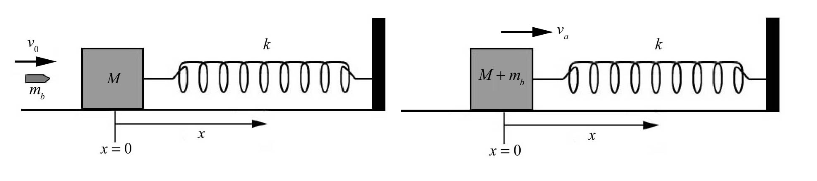
\includegraphics[scale=0.4]{2021-1/Imagenes/aux12/Captura de Pantalla 2021-06-22 a la(s) 21.45.50.png}
    %\label{fig:my_label}
\end{figure}
\begin{enumerate}
    \item Determine la velocidad del bloque inmediatamente después de que la bala impacte el bloque.
    \item El bloque se encuentra en $x=0$ cuando este comienza a moverse. Encuentre la compresión máxima del resorte.
    \item Encuentre la diferencia de energía cinética entre la $K_{bala}$ antes del impacto y $K_{bloque-bala}$ justo después del choque. 
    \item Ahora suponga que el plano no es liso, sino que se caracteriza por un coef. de roce $\mu$, y que la velocidad con la que el bloque pasa nuevamente por $x=0$ es la mitad de la encontrada en la parte (a). Determine la distancia total recorrida hasta que el bloque vuelve al punto de partida. 
    \end{enumerate}

\begin{figure}[h!]
    \centering
    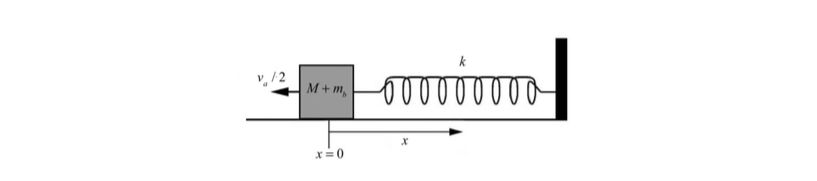
\includegraphics[scale=0.4]{2021-1/Imagenes/aux12/Captura de Pantalla 2021-06-22 a la(s) 21.46.04.png}
    %\label{fig:my_label}
\end{figure}

\item Una rueda de radio R está montada sobre un eje sin roce de manera que se mantiene vertical. Sobre el borde de la rueda se ubican tres objetos pequeños de masas $\mathbf{m}$, $\mathbf{M}$ y $\mathbf{2M}$, tal como se muestra en la figura. Determine $\mathbf{m}$ en función de $\mathbf{M}$ para que la rueda esté en equilibrio estático.

    \begin{figure}[h!]
        \centering
        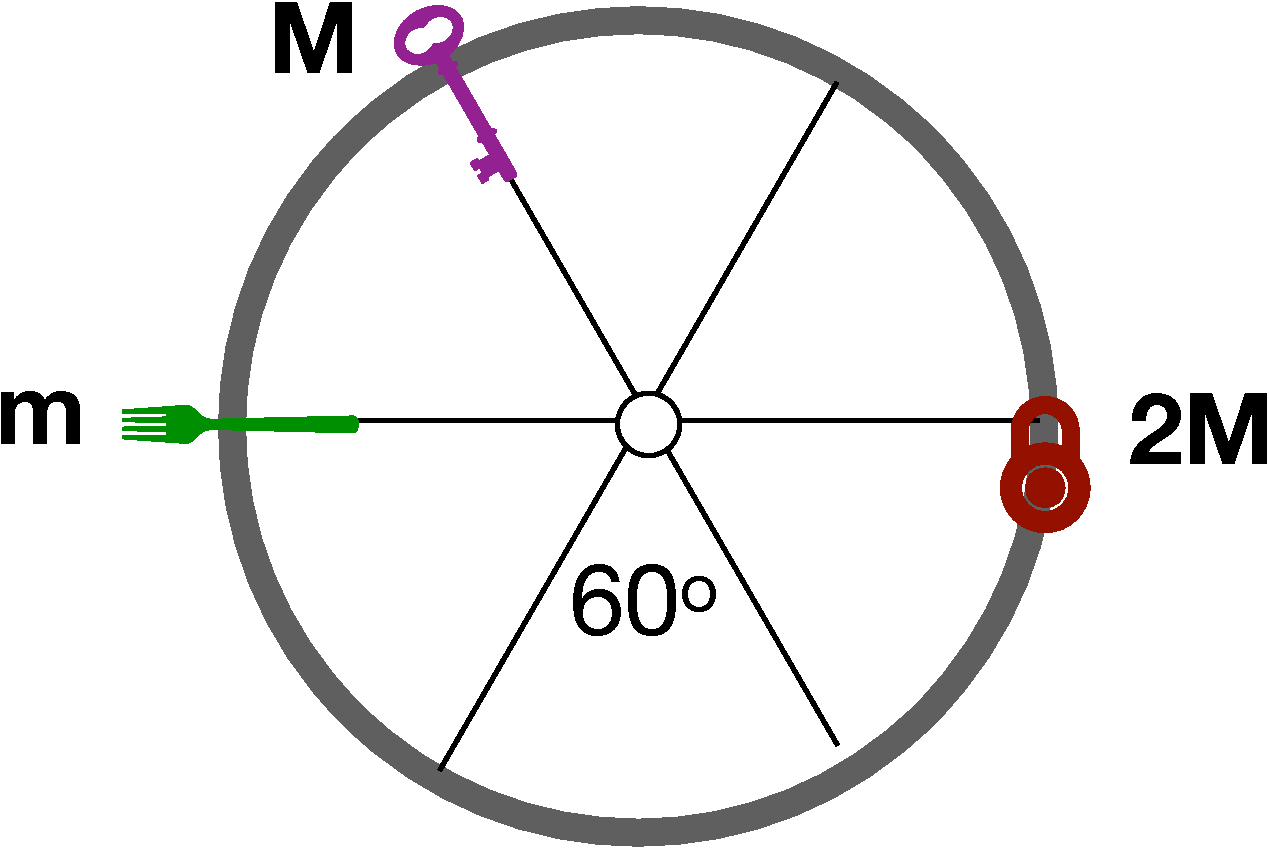
\includegraphics[scale = 0.3]{2020-1/Imágenes/ejercicios/rueda_ej12.pdf}
    \end{figure}

\end{enumerate}
\end{document}
+